

\section{Hypothesis and research questions}%
\label{sub:Hypothesis}
As \openpose is only trained on humans standing, walking, running and sitting.
The assumption in this paper is that \openpose{ } is bad at humans on the ground.
However, is that true or not?

If \openpose is as good as a human at identifying where each feature on the human is located in 2D and 3D, then a hypothesis formed such that the median and variance of both human and open pose should be equal.
Thus the hypothesis can be formed as follow:


\vspace{5mm}
\begin{align*}
    \text{H}_0: & \quad \bigmu_\text{H} = \bigmu_\text{O} \quad  \text{AND}\quad \bigsigma^2_\text{H} = \bigsigma^2_\text{O}\\
    \text{H}_1: & \quad \bigmu_\text{H} \neq \bigmu_\text{O} \quad  \text{OR}\quad \bigsigma^2_\text{H} \neq \bigsigma^2_\text{O}
\end{align*}

Where:
\begin{center}
    \begin{aligned}
        \text{H} &= \text{Human}\\
        \text{O} &= \text{OpenPose}\\
        \mu      &= \text{Median} \\
        \sigma   &= \text{Standard deviation}
    \end{aligned}
\end{center}
\bigskip
\par
The $H_0$ hypothesis states that a human and \openpose{ } are statistically similar and cannot be distinguished from each other.
If that fails, the $H_1$ hypothesis is the null hypothesis and represents no statistical difference.
But there are also a case for directional invariance between each camera location shown in~\ref{fig:camera_pos_lables}.
This can thus form an extra hypothesis that $\mu_{North}=\mu_{South}=\mu_{East}=\mu_{West}$.
Thus the hypothesis is formed such:
\vspace{5mm}
\begin{align*}
    \text{h}_0: &\quad \bigmu_\text{North}=\bigmu_\text{South} \quad\text{AND}\quad \bigmu_\text{North}=\bigmu_\text{West}\quad\text{AND}\dots\\
    \text{h}_1: &\quad \bigmu_\text{North}\neq\bigmu_\text{South} \quad\text{OR}\quad \bigmu_\text{North}\neq\bigmu_\text{West}\quad\text{OR}\dots\\
\end{align*}
In this hypothesis the $h_0$ states that the error should have a equal median value independent of rotation.
Thus if not the $h_1$ states that if that isn't the case, \openpose is not rotational invariant.

The rejection of a hypothesis is done by comparing the p-value with $\alpha=0.05$ such:
\begin{align*}
    \text{Reject H}_0 & \quad\text{if}\quad p \leq \frac{\alpha /2}{m}, \text{or}\\
    \text{Reject H}_0 & \quad\text{if}\quad 2mp \leq \alpha
\end{align*}
That last one $2mp$ is an adjusted $p$-value called a $q$-value.
Both should be less then 1 if the rejection cant be done.
But that also leads to the situation where $2mp > 1$ if $p>\alpha/m$.

\subsection{Research questions}%
\label{sub:method:research_questions}
The research questions are then derived to support those hypotheses.
\begin{itemize}
    \item[$Q_1$] Is the input distribution sufficient to reconstruct an accurate 3D pose?
    \item[$Q_2$] Can the Dijkstra/transfer method calculate the 3D position of the camera without solving the bundle adjustment problem?
    \item[$Q_3$] Is the \openpose algorithm rotational invariant around a subject on the floor.
    % \item[$Q_3$]
\end{itemize}
$Q_1$ is specified because the input distortion is larger than expected for each image, then the rest of the calculations future will increase the output error.
The Dijkstra approach perhaps does not work. Thus $Q_2$ must be specified.


In this report, the hypothesis and research questions are investigated using a minimal dataset of a human lying on the ground.
The human is lying on its side to partially hide some of the features to test how \openpose is performing with limbs occluded.
The system to create the 3D pose is presented in~\ref{sec:related_work}, but in general, it tries to use Dijkstra's algorithm to calculate the 3D position of the cameras and then the 3D pose of the feature from the cameras.
% Future more, the system uses the equation~\ref{eq:impl:muerror} to calculate the median $\mu$ for both humans and \openpose{.}
% That then forms the basis for a statistical test.


% In this paper, the proposed method to prove or disprove this hypothesis is to use a minimal data set of 21 images\ref{sec:appendices} each with several \aruco{ } corners.



% The test is done in 2D and 3D with a minimal error method using \aruco corners.
% In the end, the 3D method did not work, but sufficient validation for the hypothesis was derivable from the 2D position.
% To prove the claim that \openpose{ } was unable to find the human features accurately.
% A F-test for testing the variance and a T-test for testing the median is performed on data that is derived both from several collected data points from both human and OpenPose.\\

\subsection{Assumptions}%
\label{sub:assumptions}
The implementation uses a few assumptions to make things work.
Especially the equation~\ref{eq:impl:muerror} uses an assumption that a sample of the human population has the correct position for each label.

\noindent
Thus the assumptions in no particular order is as follow:
\begin{itemize}
    \itemize A sample of humans provide the correct position for each label, thus $\mu$ in~\ref{eq:impl:muerror} is a human sample.
\end{itemize}


\section{Method}
\label{sec:method}
From the hypotheses of this report, it is clear that the focus is on the reliability of \openpose{ } on a human subject that is lying on the ground.
That is done by comparing data from human annotations with the annotations from \operpose{} using T-test and F-test.

The general overview for how the system is used is described in figure~\ref{fig:usecase} that show how data is collected and how the results are derived from that data.

\begin{figure}
\begin{center}
    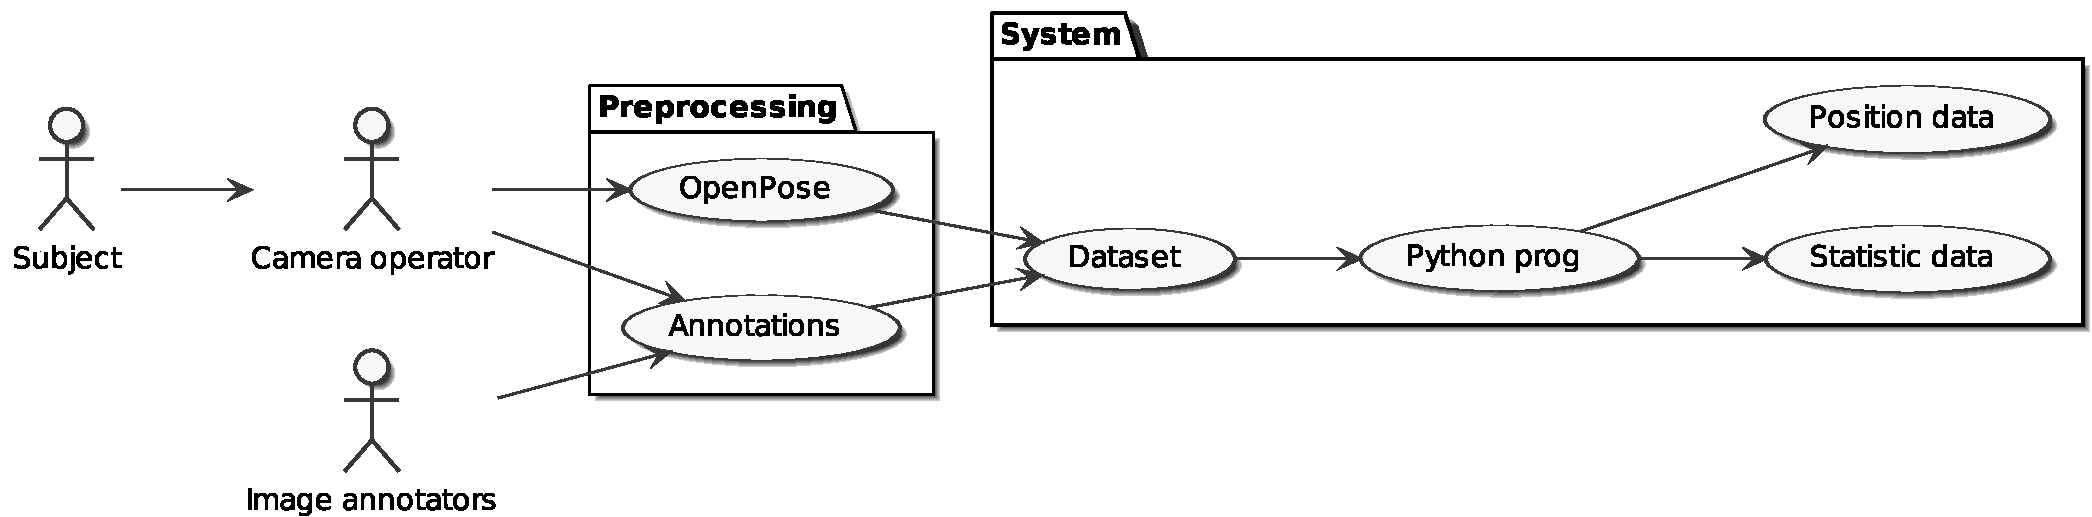
\includegraphics[scale=0.4]{figures/uml/usecase.pdf}
\end{center}
\caption{This figure shows the use case diagram for the implemented project. \textbf{Subject} on the left is the human on the ground while the \textbf{Camera Operator} is the one taking the images.
Those images are annotated by both \openpose{ } and the human \textbf{Image annotators}.
Then \openpose{ } and the annotated data is combined in to a dataset with the images.
That later are used by the implemented program to derive the \textbf{Results}}
\label{fig:usecase}
\end{figure}

Then in figure~\ref{fig:method:overview} that shows how the program is taking images and process them to become results tables covered in~\ref{sec:results} Results in more detail.

By checking with F/T-test to check if the $H_0$ hypothesis holds on the input data figure~\ref{fig:method:overview} block \textbf{2.0}.
The data can be investigated to see if the sparse 3D reconstruction could give beneficial results or not.
That is due to that sparse 3D reconstruction uses data from the input images and data.
Thus if the id does not hold, the reconstruction is probably not giving an accurate result.

The tests that are performed to prove the $H_0$ hypothesis uses the error equation~\ref{eq:impl:muerror} to calculate an error.
The error in this report is ether a \textit{label} or a \textit{direction} stated in~\ref{sub:implment:inputerror}.
The \textit{direction} error is mainly to make a simple test for how \openpose{ } reacts to having the human side upside down.
While the \textit{label} error checks how significant the error is before 3D reconstruction, that then answers the $Q_1$ question.

Regardless of the result of $Q_1$, $Q_2$  can be tested even if the result is a failed $H_0$ hypothesis if the target is not to recreate the 3D scene.
That is because the accuracy for the points does not prevent the results from the \arcuo{ } patterns to be interpreted using.

To answer the second question $Q_2$ then the system builds a pose quiver with each image and each corner in that image.
That is done in the way that was done is primarily shown in Figures~\ref{fig:camera_transfer} to~\ref{fig:multipath} and then figure~\ref{fig:method:sparce3d} expands this with a process to how this works in sequence.
However, the initial process for recovering the camera positions is done by using \aruco{ } corners spread out around the subject.
That is then done with the \aruco{ } library can then calculate the position from the camera to the \acuro{ } corners in the image.
The relative connection from corner to corner and corner to camera derives a pose quiver.

An additional test to see if there is any discrepancy for the rotation of the body is also done by manually annotating the images dependent on which quadrant
the image was taken.
That is done as proposed in~\ref{fig:camera_pos_lables} deriving the images into North, West, South and East.
The annotation, in this case, is done by the Camera Operator~\ref{fig:usecase}.





\begin{figure}
\begin{center}
    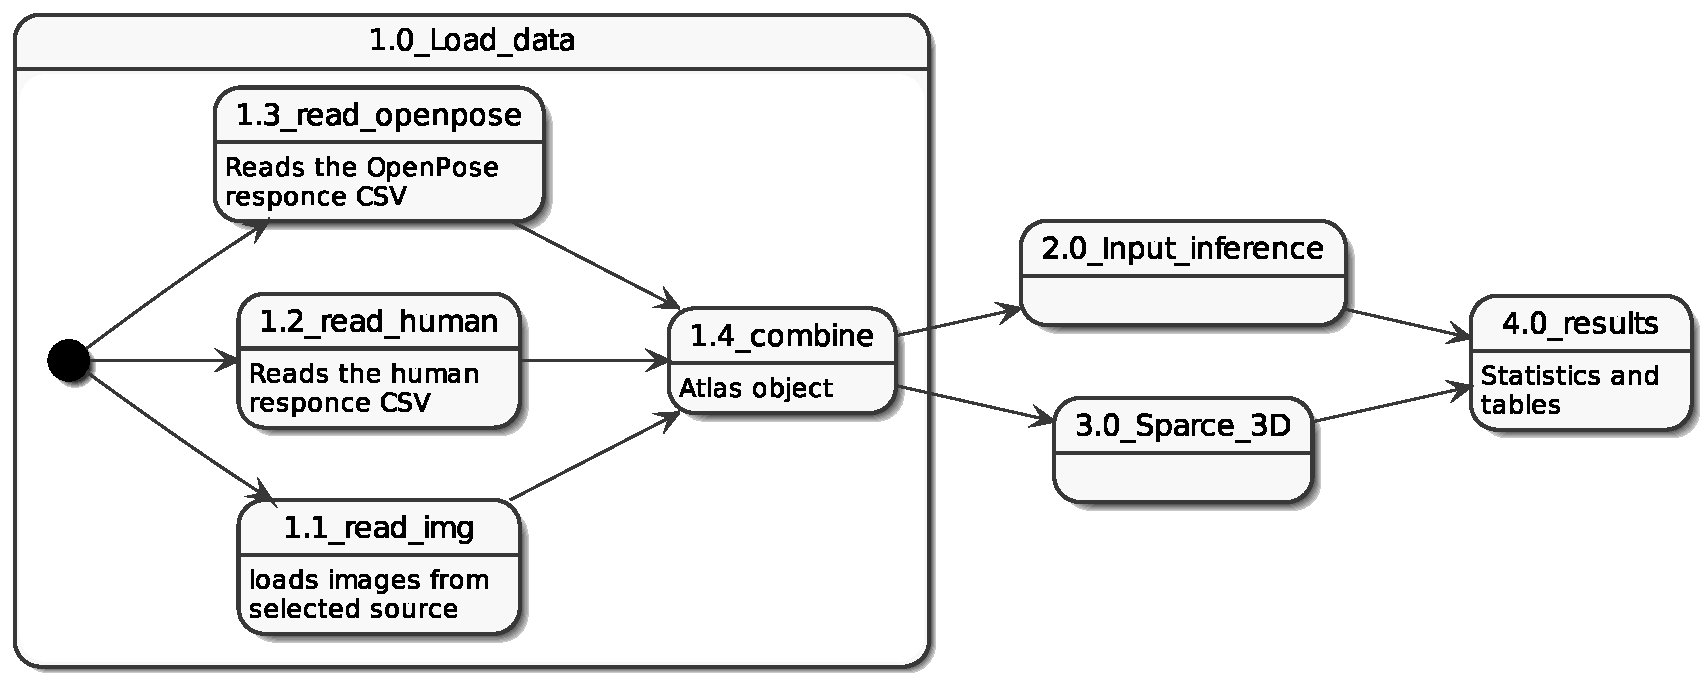
\includegraphics[scale=0.5]{figures/uml/overview.pdf}
\end{center}
\caption{This figure shows the general overview of the system created. In \textbf{1.0} loading of the images and annotated data is done.
    \textbf{2.0} Does input statistics and is future divided up in~\ref{fig:method:inference}. \textbf{3.0} does the sparce reconstruction and is divided up in~\ref{fig:method:sparce3d}.
The last part is the \textbf{4.0} results as tables shown in~\ref{sec:results}.}\label{fig:method:overview}
\end{figure}

\begin{figure}
\begin{center}
    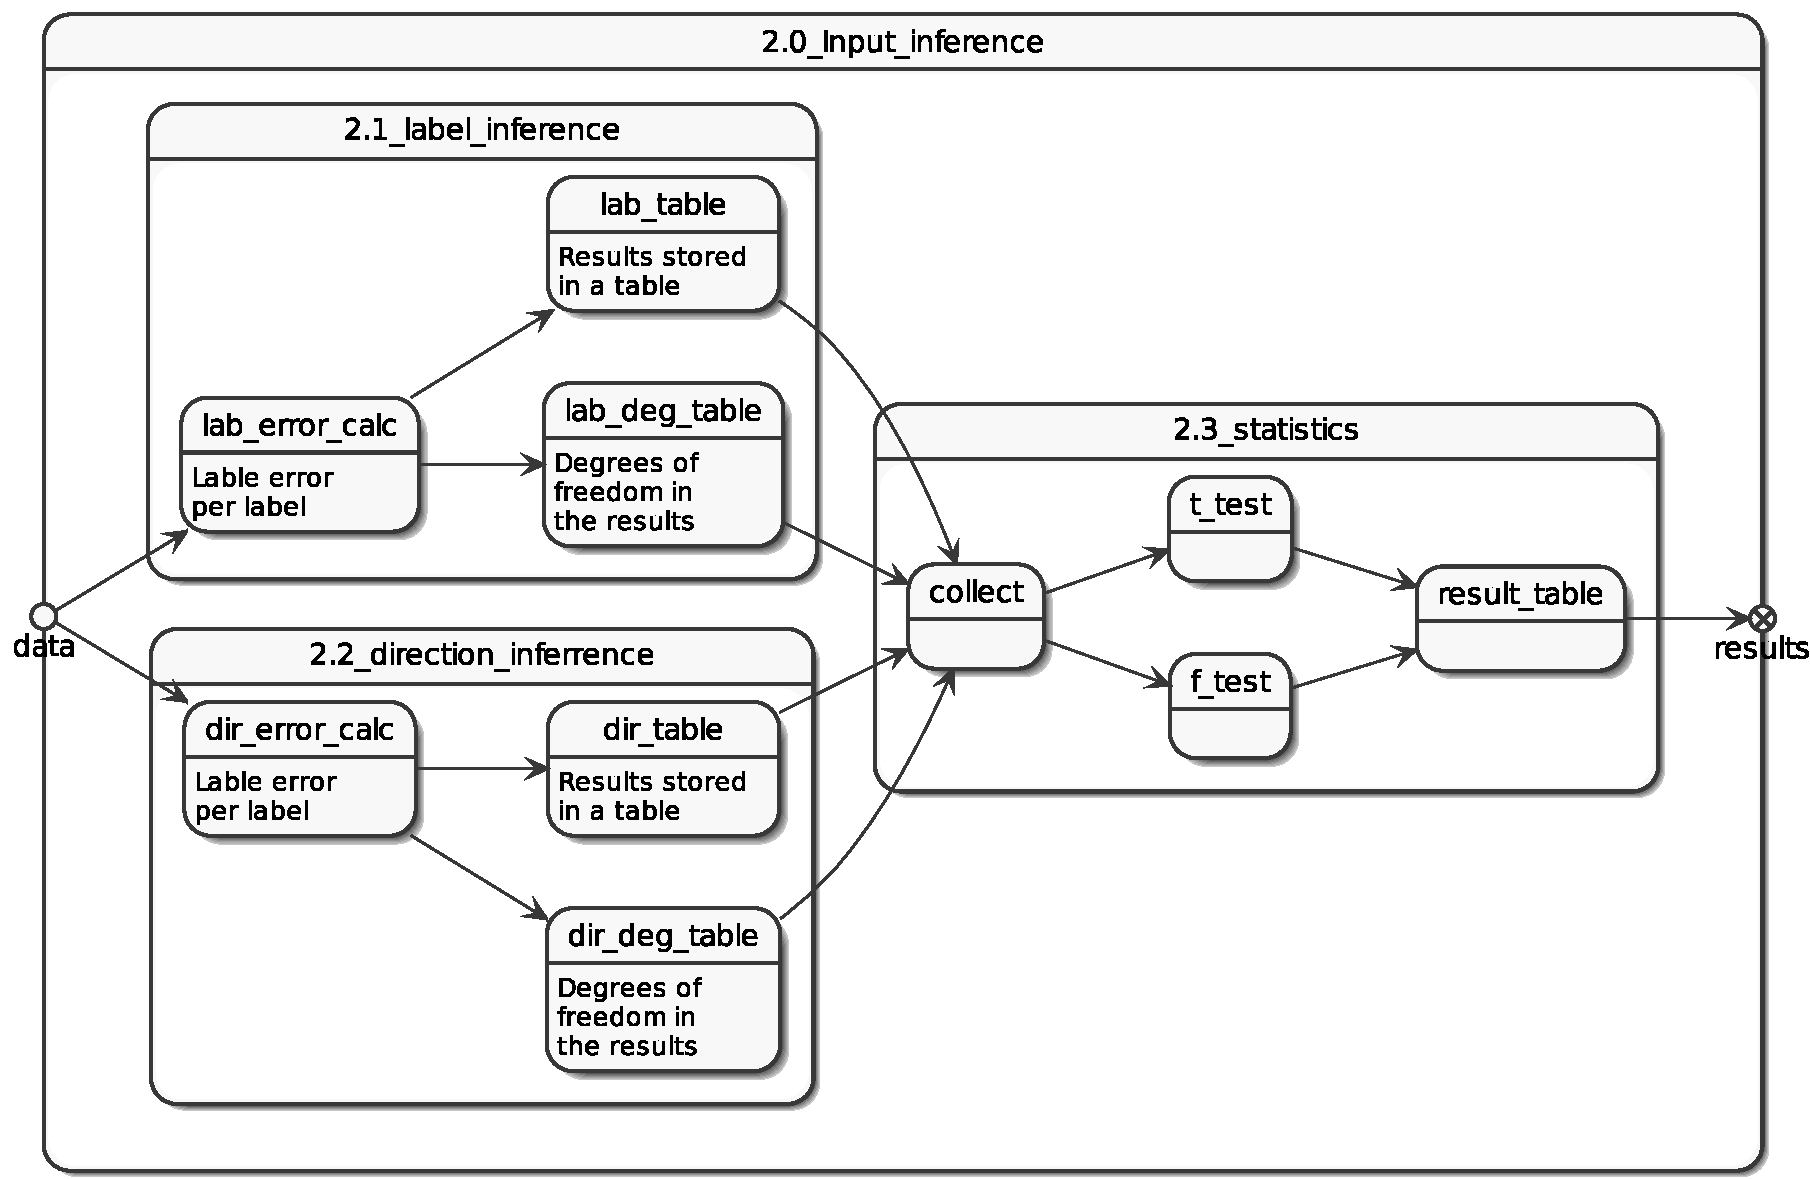
\includegraphics[scale=0.5]{figures/uml/02_input_inference.pdf}
        % 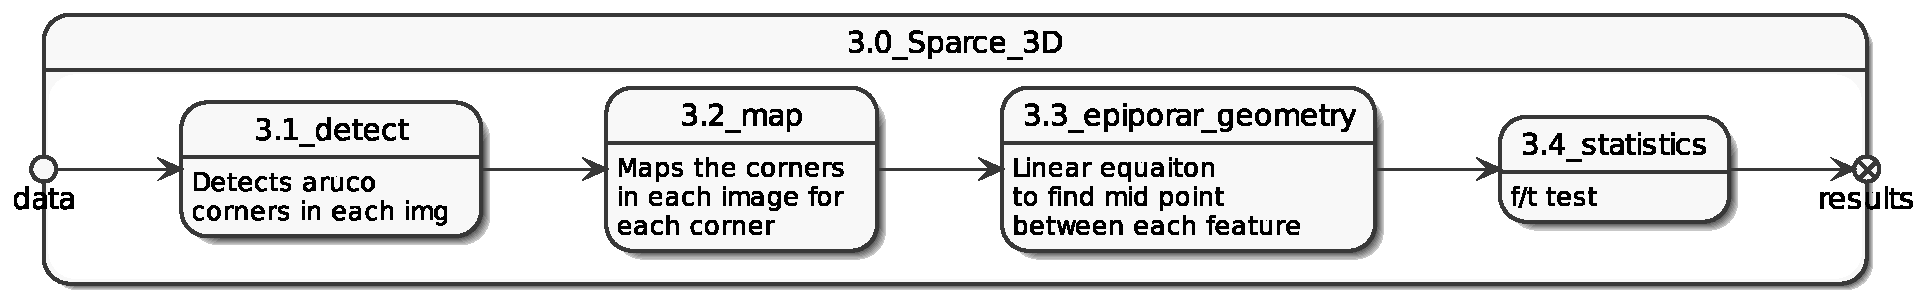
\includegraphics[scale=0.5]{figures/uml/03_sparce_3D.pdf}
\end{center}
\caption{The general overview of the input inference tests is shown in this figure.
    Both \textbf{2.1} and \textbf{2.2} uses the error function~\ref{eq:impl:muerror} and creates two tables. The first table is for labels, and the other is for degrees of freedom. That is later used in T and F tests to create a resulting table.
}
\label{fig:method:inference}
\end{figure}


\begin{figure}
    \begin{center}
        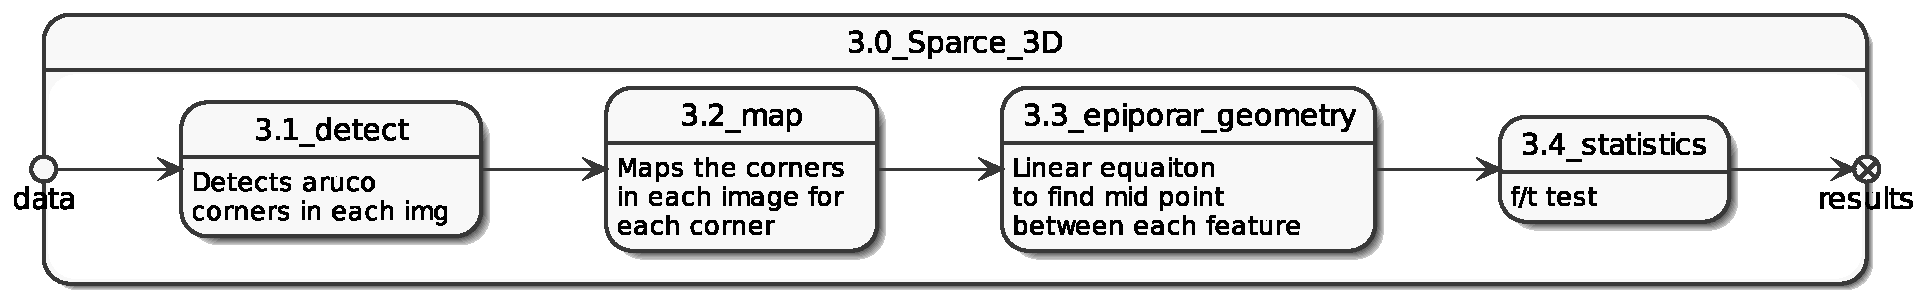
\includegraphics[scale=0.5]{figures/uml/03_sparce_3D.pdf}
    \end{center}
    \caption{The sparse 3D reconstruction shown in this overview figure begins with \textbf{3.1} detect that handles the \aruco{ } detection from each image.
        The output from that is then processed in \textbf{3.2} map node, which builds a map from each corner in each image. This step also includes the Dijkstra algorithm to calculate the shortest path from \aruco{ } origin tile to each tile and camera in the system.
        \textbf{3.3} Calculates the epipolar geometry between a set of cameras, thus deriving a point cloud for each feature in 3D space.
        Finally in \textbf{3.4} the same statistics as~\ref{fig:method:inference} \textbf{2.3} calculate the F/T-tests and derive a results table.
    }\label{fig:method:sparce3d}
\end{figure}





